\chapter{Experiments and Results}
\label{cha:ResearchAndResults}

This section will contain the results from the experiments. 

\section{Literature search}
The literature search yielded 123 studies of interest. Of these 25 had raw microRNA public. For the other studies, I sent an email requesting the raw miRNA data. However, only one such dataset were received, leading to an overall 26 datasets that are analyzed in this project (\py{", ".join(f"\\citep{{{study}}}" + ("\\footnote{\\citet{Chen2019} is not the study where the dataset originated from, but it is a study using the dataset. The dataset is GSE71661 in the Gene Expression Omnibus, and has no citation listed: \\url{https://www.ncbi.nlm.nih.gov/geo/query/acc.cgi?acc=GSE71661}}" if study == "Chen2019" else "") for study in studies)}).

The distribution of technologies in these different studies are visualized in \autoref{fig:technologies}, the number of samples are visualized in \autoref{fig:number_of_samples} and a table with the characteristics of the different datasets is in \autoref{tab:studies}.

\begin{figure}
    \centering
    \begin{tikzpicture}
        \begin{axis}[
                ybar,
                symbolic x coords={qRT-PCR, Microarrays, Sequencing},
                xtick=data,
                ylabel={Number of studies},
                ymin=0,
                ymax=20
            ]
            \addplot coordinates {(qRT-PCR, 6) (Microarrays, 16) (Sequencing, 3)};
        \end{axis}
    \end{tikzpicture}
    \caption{Number of studies of each type}
    \label{fig:technologies}
\end{figure}

\begin{figure}
    \begin{subfigure}[b]{0.25\textwidth}
        \resizebox{\textwidth}{!}{
            \begin{tikzpicture}
                \begin{axis}[
                        ybar stacked,
                        legend style={at={(0.5,-0.20)},
                        anchor=north,legend columns=-1},
                        ylabel={Number of samples},
                        reverse legend=true,
                        legend style={cells={anchor=west}, legend pos=north east},
                        table/col sep=comma,
                        ymin=0,
                        xtick=\empty,
                        %    ymode=log,
                        width=\textwidth,
                        bar width=5pt,
                        height=3\textwidth,
                        xmin=-1,
                        xmax=3
                    ]
                    \addplot [fill=green] table [y=Controls, x expr=\coordindex] {tables/samples_count.csv};
                    \addplot [fill=red] table [y=Cases, x expr=\coordindex] {tables/samples_count.csv};
                \end{axis}
            \end{tikzpicture}}
    \end{subfigure}
    \begin{subfigure}[b]{0.75\textwidth}
        \resizebox{\textwidth}{!}{
            \begin{tikzpicture}
                \begin{axis}[
                        ybar stacked,
                        legend style={at={(0.5,-0.20)},
                        anchor=north,legend columns=-1},
                        ylabel={Number of samples},
                        reverse legend=true,
                        legend style={cells={anchor=west}, legend pos=north east},
                        table/col sep=comma,
                        ymin=0,
                        xtick=\empty,
                        %    ymode=log,
                        width=\textwidth,
                        bar width=5pt,
                        height=\textwidth
                    ]
                    \addplot [fill=green] table [y=Controls, x expr=\coordindex] {tables/samples_count2.csv};
                    \addplot [fill=red] table [y=Cases, x expr=\coordindex] {tables/samples_count2.csv};
                    \legend{Controls, Cases}
                \end{axis}
            \end{tikzpicture}}
    \end{subfigure}
    \caption{The number of samples in the different studies}
    \label{fig:number_of_samples}
\end{figure}

\sisetup{round-mode=places, round-precision=3}
\begin{sidewaystable}
    \resizebox{\textwidth}{!}{
    \begin{tabular}{|r|c|c|c|c|c|c|c|}
        \hline
        \bfseries Study & \bfseries Technology & \bfseries EV (uniform) & \bfseries EV (weighted) & \bfseries \# miRNAs & \bfseries \# Cases & \bfseries \# Controls & \bfseries \# Total
        \csvreader[head to column names]{tables/studies_table.csv}{}{
            \\\citet{\Study} & \Technology & \num{\uniform} & \num{\weighted} & \mirnas & \cases & \controls & \total
        }
    \\\hline
    \end{tabular}}
    \caption{Characteristics of the studies in this project. EV=Explained Variance. Explained variance is the proportion of variance that is due to case-control characteristics (see \autoref{subsec:explained_variance}).}
    \label{tab:studies}
\end{sidewaystable}


\section{Processing the datasets}

The processing of the datasets went mostly fine, except that there were some issues due to differences in reported information about the patient characteristics. Due to that, not all datasets were adjusted for sex, age and/or packing years. Therefore, one would expect some problems regarding that not all covariates are adjusted for in all datasets, which lead to worse comparability of the datasets.


\section{Explained variance}
\label{sec:explained_variance_res}

The proportion of variance that can be attributed to case-control characteristics is shown in \autoref{tab:studies}. One interesting question is whether there is some relationship between the number of miRNA-sequences in the datasets and the proportion of variance that is due to case-control characteristics. Intuitively, there might be that studies that are more selective in the number of miRNA-sequences choose miRNA-sequences that are expected to react to case-control characteristics, and thus having a larger portion of variance due to case-control statistics. A scatter plot of the relationship between number of miRNA-sequences and the explained variance, using variance weighted explained variance, is shown in \autoref{fig:explained_variance}. Seemingly, there is no relationship. A correlation test using Pearson's r finds no significant correlation with $r=-0.24$ ($p=0.25$).
\begin{figure}
    \begin{subfigure}[b]{0.5\textwidth}
        \resizebox{\textwidth}{!}{
            \begin{tikzpicture}
                \begin{axis}[
                        xlabel={Number of miRNA sequences},
                        ylabel={Explained variance},
                        xmode=log,
                        ymode=log
                    ]
                    \addplot[
                        scatter,only marks,scatter src=x,
                        table/col sep=comma,
                        mark size=1pt,
                        scatter/use mapped color={draw=blue, fill=blue},
                    ]
                    table[x={mirna sequences},y=weighted]{tables/explained_variance.csv};
                \end{axis}
            \end{tikzpicture}
        }
        \caption{Scatter plot of explained variance and number of miRNAs.}
        \label{fig:explained_variance}
    \end{subfigure}
    \begin{subfigure}[b]{0.5\textwidth}
        \resizebox{\textwidth}{!}{
            \begin{tikzpicture}
                \begin{axis}[
                        xlabel={Number of samples},
                        ylabel={Explained variance},
                        xmode=log,
                        ymode=log
                    ]
                    \addplot[
                        scatter,only marks,scatter src=x,
                        table/col sep=comma,
                        mark size=1pt,
                        scatter/use mapped color={draw=blue, fill=blue},
                    ]
                    table[x=totals,y=weighted]{tables/explained_variance.csv};
                \end{axis}
            \end{tikzpicture}
        }
        \caption{Scatter plot of explained variance and number of samples.}
        \label{fig:explained_variance_b}
    \end{subfigure}
    \caption{Scatter plots of variance weighted explained variance.}
\end{figure}

Another possibility is that the proportion of variance is higher when there are fewer samples in the dataset. Which could suggest that the estimated case-control difference is overestimated when there are few cases, as fewer cases would lead to more overfitting. \autoref{fig:explained_variance_b} suggests a slightly negative relationship with \citet{Asakura2020} as an outlier. A correlation test using Pearson's r results in $r=-0.50$ ($p=0.01$), which suggests a negative relationship. 

\section{PCA of the datasets}

PCA plots were made for the different datasets to visualize the datasets. PCA plots for all the datasets are in \autoref{fig:pca_plots}. The datasets varies in the degrees of separation between cases and controls in the two first principal components. It also shows the general spread and clustering within the dataset. It can also be used to see the effect of the data manipulation as in \autoref{fig:pca_asakura_cleaning}.


\section{Some notes on \citet{Asakura2020}}

This is a section with some notes on \citet{Asakura2020}. There are three main reasons why there is a section for this study in particular:
\begin{itemize}
    \item It is the clearly largest dataset.
    \item It reports of a very high degree of seperation.
    \item It was a clear outlier in explained variance (see \autoref{sec:explained_variance_res})
\end{itemize}

\citet{Asakura2020} which reported virtually perfect separation (AUC $=0.996$) using two miRNAs. Looking at the dataset in the PCA-plot on unadjusted data also suggested almost perfect seperation. The miRNA-sequence that had best seperation in the study, miR-17-3p, reported a seperation of $0.935$ in the discovery set. Using the entire dataset with data preprocessing I found an AUC of $0.88$. The AUC of this miRNA in different datasets is shown in \autoref{tab:mirna_sep}. As one can see, the degree of seperation for this microRNA-sequence does not replicate well across studies, which suggest that it might be hard to get a similar seperation in other datasets, if one trains a model on the \citet{Asakura2020} dataset.

\begin{table}
    \sisetup{round-mode=places, round-precision=3}
    \begin{center}
        \csvreader[head to column names, tabular=|r|c|,
        table head = \hline \bfseries Study & \bfseries AUC\\\hline,
        late after line=\\, late after last line=\\\hline]{tables/AUC-miR-17-3p.csv}{}{
            \citet{\study} & \num{\AUC}
        }
    \end{center}
    \caption{The AUC when using miR-17-3p to diagnose lung cancer in studies where miR-17-3p is measured}
    \label{tab:mirna_sep}
\end{table}

\begin{figure}
    \begin{subfigure}[b]{0.5\textwidth}
        \resizebox{\textwidth}{!}{
            \begin{tikzpicture}
                \begin{axis}[
                        xlabel={Principal Component 1},
                        ylabel={Principal Component 2},
                    ]
                    \addplot[
                        scatter,only marks,scatter src=explicit symbolic,
                        scatter/classes={
                            Control={green},
                            Cancer={red}
                        },
                        table/col sep=comma,
                        mark size=1pt
                    ]
                    table[x=PCA1,y=PCA2,meta=Type]{tables/PCA/Asakura2020_old.csv};
                    \legend{Control,Cancer}
                \end{axis}
            \end{tikzpicture}}
        \caption{PCA of \citet{Asakura2020} before covariates were adjusted for and before post operation samples were removed}
        \label{fig:pca_asakure_non_cleaned}
    \end{subfigure}
    \begin{subfigure}[b]{0.5\textwidth}
        \resizebox{\textwidth}{!}{
            \begin{tikzpicture}
                \begin{axis}[
                        xlabel={Principal Component 1},
                        ylabel={Principal Component 2},
                    ]
                    \addplot[
                        scatter,only marks,scatter src=explicit symbolic,
                        scatter/classes={
                            Control={green},
                            Cancer={red}
                        },
                        table/col sep=comma,
                        mark size=1pt
                    ]
                    table[x=PCA1,y=PCA2,meta=Type]{tables/PCA/Asakura2020.csv};
                    \legend{Control,Cancer}
                \end{axis}
            \end{tikzpicture}}
        \caption{PCA of \citet{Asakura2020} after covariates have been adjusted for and with post operation samples removed}
        \label{fig:pca_asakura_cleaned}
    \end{subfigure}
    \caption{The PCA plots show the effect of data cleaning in \citet{Asakura2020}}
    \label{fig:pca_asakura_cleaning}
\end{figure}

\autoref{fig:pca_asakura_cleaning} shows that a lot of the separation between cases and controls in the dataset is due to different demographics. This makes the data harder to make inference on, as the two groups are not directly comparable. If the effect of the demographic variables is not linear, which is a reasonable assumption, the adjustment done will not control for demographic effects fully, leading to worse results than what would be the case if cases and controls were more similar demographically.

\section{Log-fold-change correlation} 
Log-fold-change correlations were calculated between the datasets in order to see to what degree differences between cases and controls replicate across datasets. To ensure that the correlations were significant, p-values were calculated. As controls, p-values were also calculated the columns representing the different miRNA-sequences were shuffled and when samples were randomly assigned to case and control. This is visualized in \autoref{fig:log_fold_change_correlation_pvalues}.

\begin{figure}
    \begin{subfigure}[b]{0.5\textwidth}
        \resizebox{\textwidth}{!}{
            \begin{tikzpicture}
                \begin{axis}[
                        xlabel={p-value},
                        ylabel={Count},
                        ybar,
                        ymin=0
                    ]
                    \addplot[
                        hist = {
                            bins=10,
                            data min=0,
                            data max=1
                        },
                        table/col sep=comma,
                        fill=blue
                    ]
                    table[y=real]{tables/log_fold_change_pvalues.csv};
                \end{axis}
            \end{tikzpicture}
        }
        \caption{p-values for log-fold-change correlation for when doing no manipulations}
        \label{fig:fold_correlation_pvalues_real}
    \end{subfigure}
    \begin{subfigure}[b]{0.5\textwidth}
        \resizebox{\textwidth}{!}{
            \begin{tikzpicture}
                \begin{axis}[
                        xlabel={p-value},
                        ylabel={Count},
                        ybar,
                        ymin=0
                    ]
                    \addplot[
                        hist = {
                            bins=10,
                            data min=0,
                            data max=1
                        },
                        table/col sep=comma,
                        fill=blue
                    ]
                    table[y={mirna-shuffled}]{tables/log_fold_change_pvalues.csv};
                \end{axis}
            \end{tikzpicture}
        }
        \caption{p-values for log-fold-change correlation when the order of the columns with miRNA-sequences are shuffled}
        \label{fig:fold_correlation_pvalues_mirna_shuffled}
    \end{subfigure}
    \begin{subfigure}[b]{0.5\textwidth}
        \resizebox{\textwidth}{!}{
            \begin{tikzpicture}
                \begin{axis}[
                        xlabel={p-value},
                        ylabel={Count},
                        ybar,
                        ymin=0
                    ]
                    \addplot[
                        hist = {
                            bins=10,
                            data min=0,
                            data max=1
                        },
                        table/col sep=comma,
                        fill=blue
                    ]
                    table[y={case-shuffled}]{tables/log_fold_change_pvalues.csv};
                \end{axis}
            \end{tikzpicture}
        }
        \caption{p-values for log-fold-change correlation when case-control is randomly assigned}
        \label{fig:fold_correlation_pvalues_case_shuffled}
    \end{subfigure}
    \caption{p-values for the correlations when doing different manipulations of the data}
    \label{fig:log_fold_change_correlation_pvalues}
\end{figure}

As one can see, the correlations were much more significant when the miRNA-sequences were not shuffled, which means there are at least some consistencies across the datasets. However, that correlations have similar significance whether I use real or random case-control suggests that the case-control differences might not replicate across studies.

The size of the correlations were, however, not very promising as the correlations were poor, and in many cases negative. The correlations of the log-fold-changes are mostly small, and the correlations are often negative, as shown in \autoref{fig:log_fold_change_correlations}. Even as these correlations are small and centered around zero, they are not spurious as shown with the p-values in \autoref{fig:log_fold_change_correlation_pvalues}. However, as p-values were similar when case-control characteristics were randomly assigned, this might suggest that the correlations are due to covariance between different miRNA-sequences rather than having to do with case-control characteristics.

\begin{figure}
    \centering
    \begin{tikzpicture}
        \begin{axis}[
                xlabel={Correlation},
                ylabel={Count},
                ybar,
                ymin=0
            ]
            \addplot[
                hist = {
                    bins=30,
                    data min=-1,
                    data max=1
                },
                table/col sep=comma,
                fill=blue
            ]
            table[y=correlations]{tables/log_fold_change_correlations.csv};
        \end{axis}
    \end{tikzpicture}
    \caption{Histogram of the correlation in log-fold-change between the studies.}
    \label{fig:log_fold_change_correlations}
\end{figure}

An overview over all the log-fold-change correlations is in \autoref{tab:log_fold_table}.

\subsection{Graph analysis of log-fold-change correlations}

It is interesting to see whether there are any pattern in what studies correlates with other studies. I plotted a graph where there is an edge between two datasets iff they have at least 10 miRNA-sequences in common and the log-fold-change correlation is significant at a 0.05 significance level. The graph is in \autoref{fig:fold-change-graph}. There are clearly some studies that correlates with many other studies, and others that are outliers. Studies that are outliers would probably be difficult to use to diagnose in other datasets.

\begin{figure}
    \centering
    \includesvg[width=\textwidth]{figs/fold-change-graph}
    \caption{Graph over the log-fold-change correlation. The size of the nodes is proportional to the logarithm of number of cases in the datasets.}
    \label{fig:fold-change-graph}
\end{figure}


\section{Machine learning on the datasets}

Machine learning was done where a logistic regression model was trained on one dataset and used to predict on another dataset. In \autoref{fig:auc_values} the AUC values are shown, but only for pair of datasets with at least 10 different miRNA-sequences in common.
The AUCs are close to 0.5, which means that there is little predictive power in general.
\autoref{tab:cross_auc} contains all the AUCs for the different datasets.

\begin{figure}
    \centering
    \begin{tikzpicture}
        \begin{axis}[
                xlabel={AUC},
                ylabel={Count},
                ybar,
                ymin=0
            ]
            \addplot[
                hist = {
                    bins=25,
                    data min=0,
                    data max=1
                },
                table/col sep=comma,
                fill=blue
            ]
            table[y=auc]{tables/auc_histogram.csv};
        \end{axis}
    \end{tikzpicture}
    \caption{Histogram of the AUC when training on one study and predicting on another study.}
    \label{fig:auc_values}
\end{figure}


\subsection{Clique analysis of machine learning results}
Post hoc, it seemed interesting to see if there is some transitivity in whether datasets can be used to predict each other. I.e. if a model trained on dataset A can diagnose well in a dataset B, and a model trained on B can diagnose well in dataset C, does that imply that a model trained on A can predict well on C? For this analysis a graph was made that had a edge between dataset A and B iff they had at least 10 miRNA-sequences in common and the AUC of the model trained on A predicting on  B was greater than 0.6 and same with the model trained on B predicting on A. This graph is shown in \autoref{fig:graph}. Then the problem became to find the maximal cliques in the resulting graph. The maximum clique that was found in the graph consisted of \citet{Duan2021}, \citet{Keller2020}, \citet{Jin2017} and \citet{Halvorsen2016}.


\begin{figure}
    \centering
    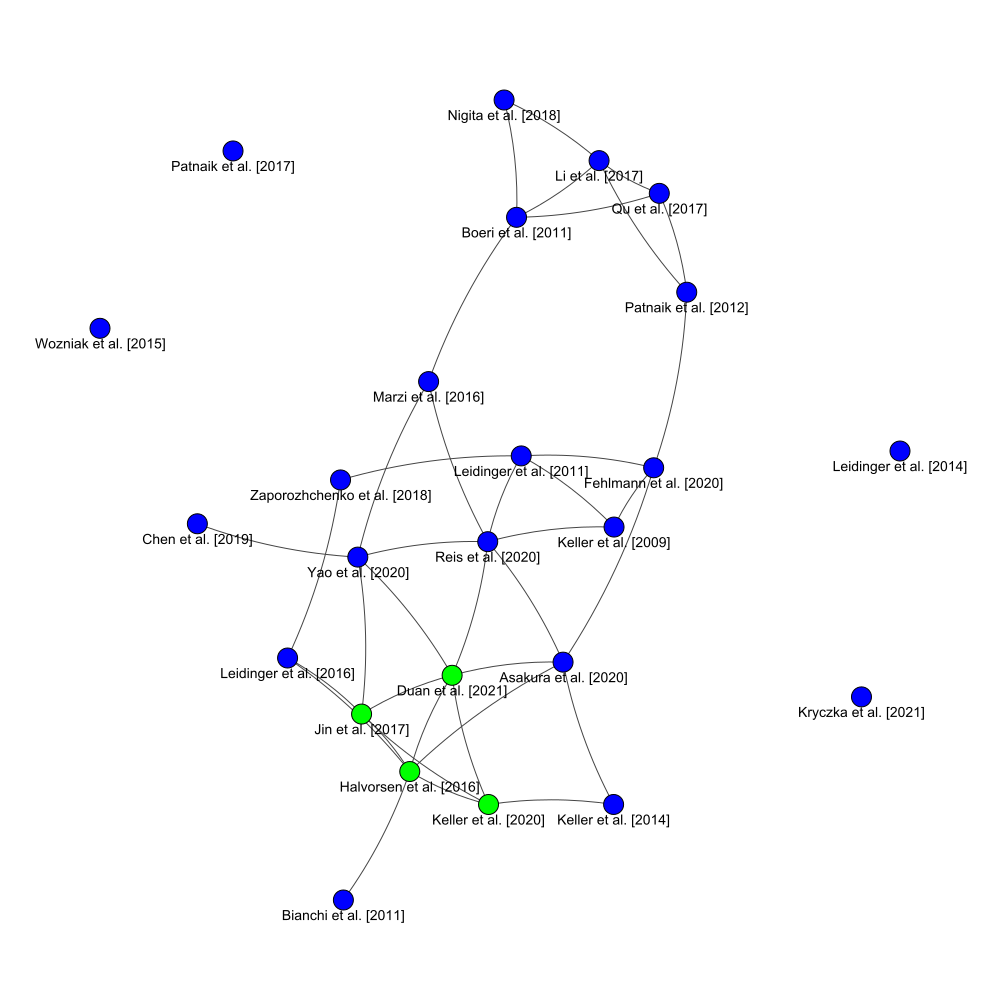
\includegraphics[width=\textwidth]{figs/graph}
    \caption{Graph over the datasets. The maximum clique is marked in green.}
    \label{fig:graph}
\end{figure}

\iffalse
\begin{figure}
    \usetikzlibrary {graphs,graphdrawing} \usegdlibrary {force}
    \begin{pycode}
print("""\\resizebox{\\textwidth}{!}{""")
print("""\\tikz \\graph [random seed=11, spring electrical layout, nodes={draw, rectangle}, node distance=4.25cm] {""")

import pandas as pd
data = pd.read_csv("tables/CrossAUC.csv", index_col=0)
data.replace("*", 0, inplace=True)
data = data.apply(pd.to_numeric)
data = data > 0.6
max_clique = ['Duan2021', 'Keller2020', 'Jin2017', 'Halvorsen2016']
for study in studies:
    print(f""""\\citet{{{study}}}" {"[fill=green]" if study in max_clique else ""};""")
for i, s1 in enumerate(studies):
    for s2 in studies[i+1:]:
        if data[s1][s2] * data[s2][s1]:
            print(f""""\\citet{{{s1}}}" -- "\\citet{{{s2}}}";""")
print("""};}""")
    \end{pycode}
\end{figure}
\fi

\iffalse

\section{Experimental Plan}
\label{sec:experimentalPlan}

Trying and failing is a major part of research. However, to have a chance of success you need a plan driving the experimental research, just as you need a plan for your literature search. Further, plans are made to be revised and this revision ensures that any further decisions made are in line with the work already completed.  

The plan should include what experiments or series of experiments are planned and what question the individual or set of experiments aim to answer. Such questions should be connected to your research questions so that in the evaluation of your results you can discuss the results wrt to the research questions.  

\section{Experimental Setup}
\label{sec:experimentalSetup}

The experimental setup should include all data - parameters etc, that would allow a person to repeat your experiments. 

\section{Experimental Results}
\label{sec:experimentalResults}

Results should be clearly displayed and should provide a suitable representation of your results for the points you wish to make. Graphs should be labeled in a legible font and if more than one result is displayed on the same graph then these should be clearly marked.   Please choose carefully rather than presenting every results. Too much information is hard to read and often hides the key information you wish to present. Make use of statistical methods when presenting results, where possible to strengthen the results.  Further, the format of the presentation of results should be chosen based on what issues in the results you wish to highlight. You may wish to present a subset in the experimental section and provide additional results in the appendix.

\fi
